\documentclass[AutoFakeBold]{ctexart}
\usepackage{physics_report}

% Essential!!!
% Only for test, delete when use this template!
\usepackage{lipsum, color}


\title{光学模块实验报告}
\author{author1\superscript{1)} \quad author2\superscript{1)} }
\institude{1)中山大学物理学院,广州 510275}
\engtit{Report of Optics Experiment}
\engauth{J.H. He\comauthor{1)} \quad Y.C. Guo\superscript{1)} \quad W. He\superscript{1)} \quad J.J. He\superscript{1)}}
\engins{1)School of physics, Sun Yet-Sen University, Guangzhou 510275, China}




\begin{document}

    \maketitle
    \abstract{这是一小段摘要}
    \keywords{微波,波导,晶体}
    \pacs{95.85.Bh, 84.40.Az, 02.60.Ed}

    \zihao{-4}这些是小四号的字吗
        
    % \columnseprule=1pt         % 实现插入分隔线 
    \begin{multicols}{2}
        \section{第一节}
        \subsection{小测试}
        \textcolor{red}{使用者请注意:}前面配上一段文字,配合使用\textbackslash\textbackslash 效果更佳,就像这样\\
        \begin{tabu}{\linewidth}{|X[1,c]|X[2,c]|X[3,c]|}
            A & B & C \\
            \hline
            1 & 2 & 3
        \end{tabu}

        \textcolor{red}{使用者请注意:}或者包在table环境里使用!
        \begin{table}[H]
            \begin{tabu}{\linewidth}{|X[1,c]|X[2,c]|X[3,c]|X[2,c]|X[1,c]|}
                A & BB & CCC & BB & A\\
                \hline
                1 & 22 & 333 & 22 & 1\\
            \end{tabu}
        \end{table}

        \textcolor{red}{使用者请注意:}双栏模式中一个最大的问题是,无法将占两栏图表放在当前页的底部,即使有足够的空间!!!!折中的办法是放在下一页的开头
        \begin{table*}[hbtp]
            \begin{tblr}{
                width = \linewidth,
                colspec = {X[2.5,c,m]|X[1,c,m]X[1,c,m]X[1,c,m]X[1,c,m]X[1,c,m]X[1,c,m]X[1,c,m]X[1,c,m]X[1,c,m]}
            }
            \toprule
            $I/\si{\milli\ampere}$ & 20    & 30    & 40    & 50    & 60    & 70    & 80    & 90    & 100 \\
            \midrule
            $U_2/\si{V}$ & 0.56  & 1.84  & 3.86  & 5.56  & 3.4   & 1.88  & 0.92  & 0.52  & 0.28 \\
            $U_1/\si{V}$ & 7.88  & 7.6   & 6.92  & 5.8   & 6.68  & 7     & 7.24  & 7.24  & 7.16 \\
            \bottomrule
            \end{tblr}
        \end{table*}

        \lipsum[1]
        
        \textcolor{red}{使用者请注意:}在双栏模式下,可能存在本页面无法放入图(表)的情况,会自动拉宽文字间距,将图(表)放到下一页,需注意排版!!!

        \textcolor{red}{使用者请注意:}但我们可以将想放在底部的两栏的表放在本页的开头或上一页的结尾,就能实现!!!
        \begin{table*}[hb]
            \begin{tblr}{
                width = \linewidth,
                colspec = {X[2.5,c,m]|X[1,c,m]X[1,c,m]X[1,c,m]X[1,c,m]X[1,c,m]X[1,c,m]X[1,c,m]X[1,c,m]X[1,c,m]}
            }
            \toprule
            $I/\si{\milli\ampere}$ & 20    & 30    & 40    & 50    & 60    & 70    & 80    & 90    & 100 \\
            \midrule
            $U_2/\si{V}$ & 0.56  & 1.84  & 3.86  & 5.56  & 3.4   & 1.88  & 0.92  & 0.52  & 0.28 \\
            $U_1/\si{V}$ & 7.88  & 7.6   & 6.92  & 5.8   & 6.68  & 7     & 7.24  & 7.24  & 7.16 \\
            \bottomrule
            \end{tblr}
        \end{table*}

        \section{测试图表}
        \begin{figure}[H]
            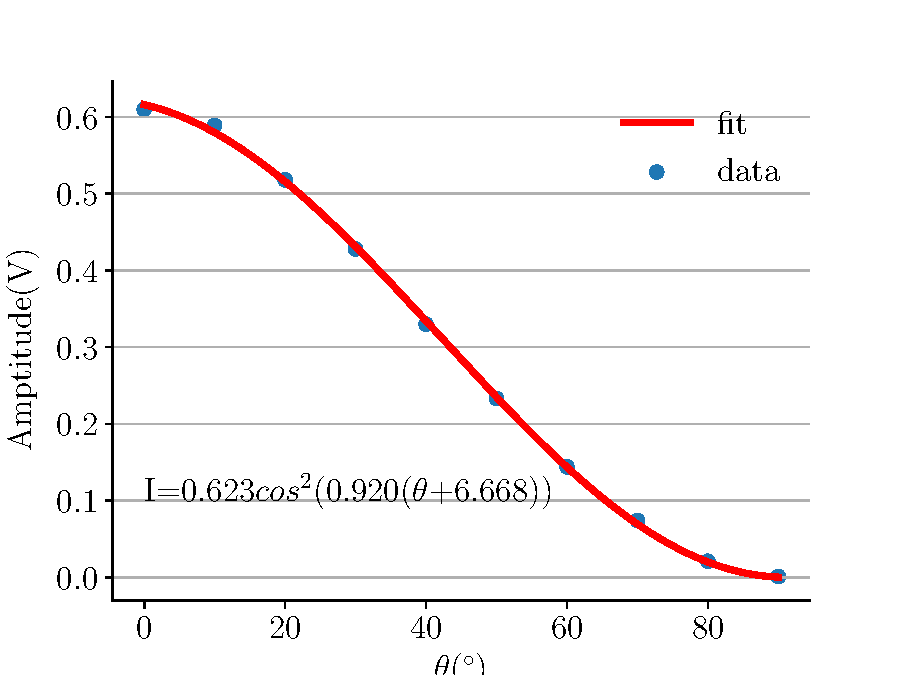
\includegraphics[width=\linewidth]{angle.eps}
            \bicaption{一个图}{a picture}\label{fig:a}
        \end{figure}
        \begin{table}[H]
            \begin{tblr}{
                width = \linewidth,
                colspec = {XXX}
            }
                \hline
                \SetCell[r=2,c=2]{c} % 直接设置合并单元格 2行2列 水平垂直居中
                合并的格子 & ~ & % 合并后的格子必须保留 “&” 并空置
                独立的格子1 \\
        
                \cline{2-3}
                ~ & ~ & 独立的格子2 \\
                \hline 
            \end{tblr}
            \bicaption{一个表}{a table}\label{tab:a}
        \end{table}

        I have made a picture pic.\ref{fig:a} and a table tab.\ref{tab:a}.
    \end{multicols}
    
    %  \begin{longtabu}{
    %     width = .8\textwidth,
    %     colspec = {XXX}
    % }
    %     A & B & C \\
    %     1 & 2 & 3
    % \end{longtabu}
   

    \bibreference[nocite]{ref}
    \makeenglishtitle
    \abstract[english]{
        \qquad \lipsum[2]
    }
    \keywords[english]{microwave, waveguide, lattice}
    
    

\end{document}

